\documentclass[11pt,a4paper]{article}
\usepackage[utf8]{inputenc}
\usepackage[T1]{fontenc}
\usepackage{amsmath, amssymb}
\usepackage{graphicx}
\usepackage{float}
\usepackage{geometry}
\geometry{margin=1in}

\title{Lab 4: Simulation in Quantum Mechanics}
\author{Gemini CLI}
\date{\today}

\begin{document}

\maketitle

\section*{1}
We simulated the interference of a Gaussian wave packet colliding with an infinite potential wall using different number of mesh points $N \in \{2^{13}, 2^{14}\}$. The figures below show the interference patterns at $t=95$.

\begin{figure}[H]
    \centering
    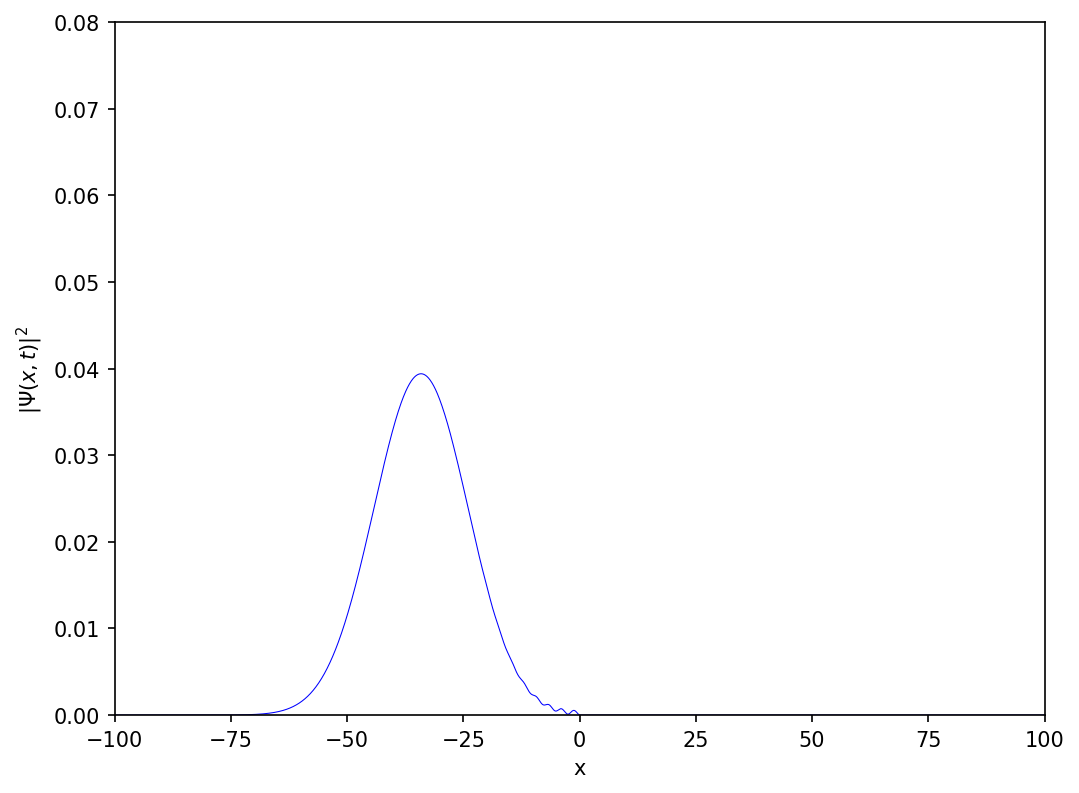
\includegraphics[width=0.7\textwidth]{task1_N8192.png}
    \caption{Interference pattern for $N = 2^{13}$}
\end{figure}

\begin{figure}[H]
    \centering
    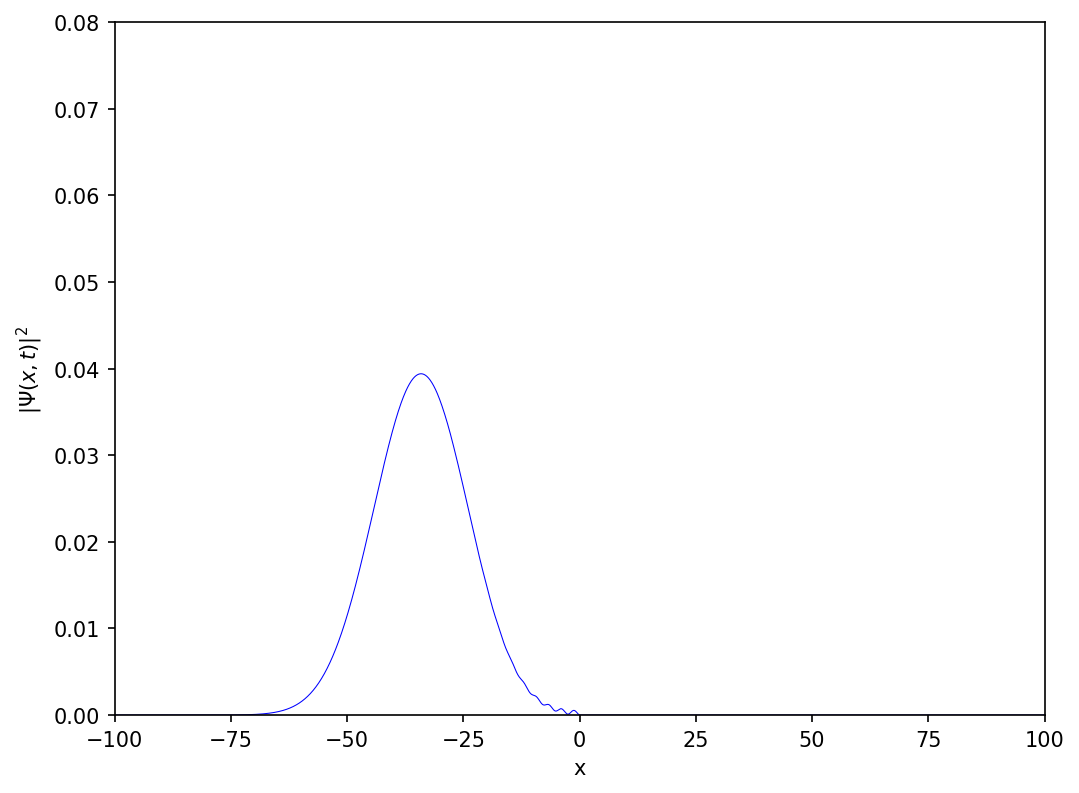
\includegraphics[width=0.7\textwidth]{task1_N16384.png}
    \caption{Interference pattern for $N = 2^{14}$}
\end{figure}

The figures for $N = 2^{13}$ and $N = 2^{14}$ are nearly identical. This suggests that the interference results are physical and not a consequence of discretization or numerical parameters.

\section*{2}
We simulated the wave packet's interaction with the Coulomb barrier potential, defined as $V(x) = 0$ for $x < 1$ and $V(x) = 1/x$ for $x \geq 1$. Figure 3 shows the probability density as the wave packet split into reflected and transmitted parts.

\begin{figure}[H]
    \centering
    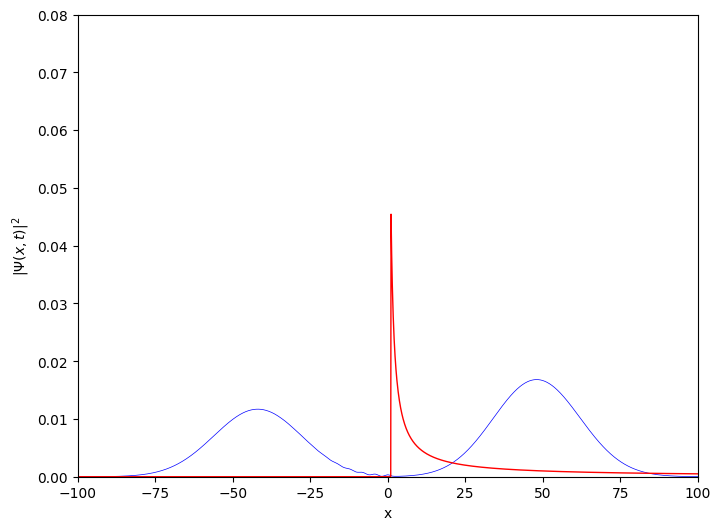
\includegraphics[width=0.7\textwidth]{task2_sim.png}
    \caption{Wave packet splitting at the Coulomb barrier ($E=0.5$)}
\end{figure}

To calculate the transmission probability $T$, we use the relation:
\begin{equation}
T = \frac{Y_T}{Y_R + Y_T}
\end{equation}
where $Y_R$ and $Y_T$ are the integrated probability densities (or maximum amplitudes in a steady state, but here we use the integrated area) for the reflected and transmitted parts respectively. According to Gamow's theory, $T$ should vary exponentially with energy $E$:
\begin{equation}
T \propto \exp\left(-\frac{k}{\sqrt{E}}\right)
\end{equation}
We plotted $\ln T$ against $1/\sqrt{E}$ in Figure 4.

\begin{figure}[H]
    \centering
    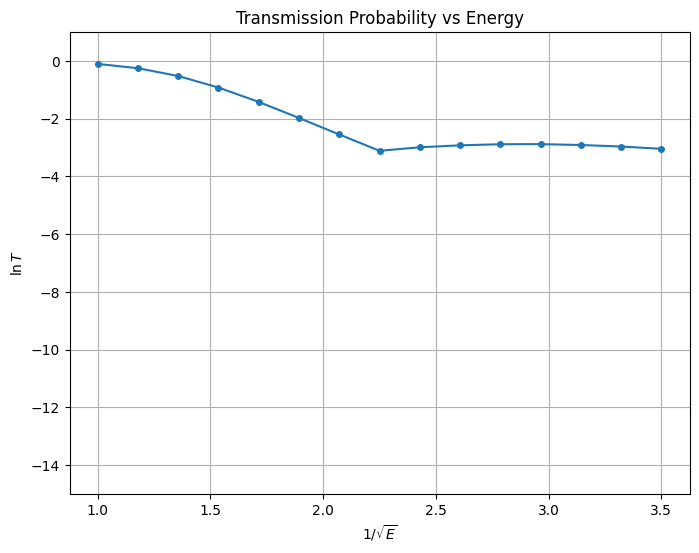
\includegraphics[width=0.7\textwidth]{task2_gamow_plot.png}
    \caption{Transmission probability vs $1/\sqrt{E}$}
\end{figure}

The plot shows a linear relationship for the investigated range, agreeing with Gamow's theoretical prediction.

\section*{3}
We initialized a Gaussian wave packet with energy $E=0.5$ (incident wave vector $k_0=1$). The potential step was defined as $V(x) = 0$ for $x < 0$ and $V(x) = 1$ for $x \geq 0$.

\begin{figure}[H]
    \centering
    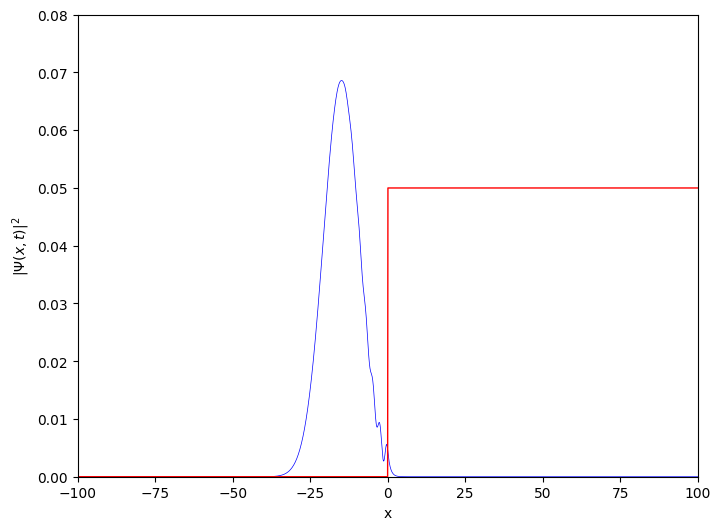
\includegraphics[width=0.7\textwidth]{task3_step.png}
    \caption{Reflection from a potential step ($E < V_0$)}
\end{figure}

As seen in Figure 5, since the energy $E=0.5$ is less than the barrier height $V_0 = 1$, the wave packet is almost entirely reflected.

Next, we applied an electric field along the x-direction, resulting in a triangular potential barrier $V(x) = V_0(1 - x/L)$ for $0 < x < L$ and $V(x) = 0$ otherwise, with $L=4$. We plotted $\ln T$ against $V_0^{3/2}$ for $V_0 \in \{0.6, 0.7, \dots, 1.2\}$.

\begin{figure}[H]
    \centering
    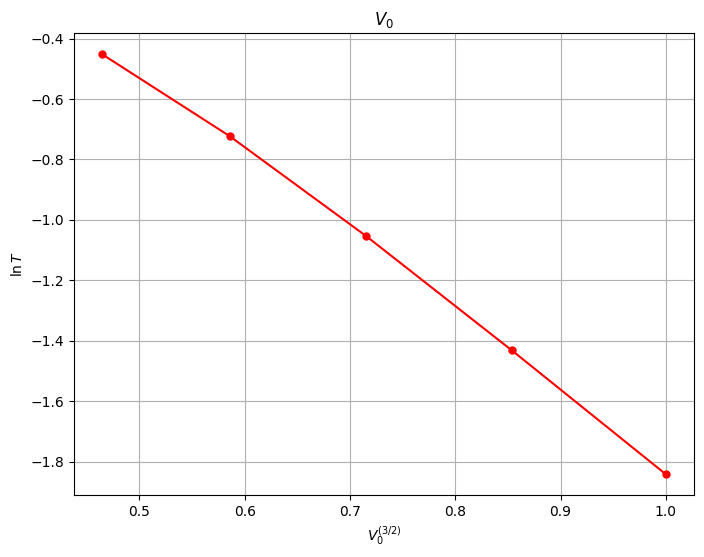
\includegraphics[width=0.7\textwidth]{task3_fn_plot.png}
    \caption{$\ln T$ vs $V_0^{3/2}$ for Fowler-Nordheim tunneling}
\end{figure}

The linear relationship in Figure 6 agrees with the WKB approximation for field emission, where the transmission probability decreases exponentially with $V_0^{3/2}$.

\end{document}
